\documentclass{article}
\usepackage{amsmath}
\usepackage{amssymb}
\usepackage{tikz}

\begin{document}

\section*{Monomorphisms in Category Theory}

\subsection*{Definition}
A morphism $f : A \rightarrow B$ in a category $\mathcal{C}$ is called a \textbf{monomorphism} (or \textbf{mono}) if for every pair of morphisms $g, h : C \rightarrow A$, the condition $f \circ g = f \circ h$ implies $g = h$.
\newline
In symbols:
\begin{equation*}
\forall g, h : C \rightarrow A, \quad (f \circ g = f \circ h) \implies (g = h)
\end{equation*}

\subsection*{Key Properties of Monomorphisms}
\begin{itemize}
    \item \textbf{Left Cancellative}: Monomorphisms are left cancellative. This means that if $f \circ g = f \circ h$ and $f$ is a monomorphism, then $g = h$.
    \item \textbf{Generalization of Injective Functions}: In the category of sets, a monomorphism corresponds to an injective (one-to-one) function. However, in other categories, the notion of a monomorphism might not coincide with injectivity in the usual sense.
    \item \textbf{Stability Under Composition}:
    \begin{itemize}
        \item If $f : A \rightarrow B$ and $g : B \rightarrow C$ are monomorphisms, then the composition $g \circ f : A \rightarrow C$ is also a monomorphism.
    \end{itemize}
\end{itemize}

\subsection*{Diagrams}
\subsubsection{External diagram}
Given that $f$ is a monomorphism,
\begin{equation*}
    f \circ g = f \circ h \implies g = h
\end{equation*}

\begin{center}
\begin{tikzpicture}[node distance=3cm, auto]
  % Nodes
  \node (C) at (0, 0) {$C$};
  \node (A) at (3, 2) {$A$};
  \node (B) at (6, 0) {$B$};

  % Arrows
  \draw[->] (C) to node [swap] {$g$} (A);
  \draw[->] (C) to node {$h$} (A);
  \draw[->] (A) to node {$f$} (B);

  % Arrow compositions
  \draw[->, dashed] (C) to node [swap] {$f \circ g$} (B);
  \draw[->, dashed] (C) to node {$f \circ h$} (B);
\end{tikzpicture}

\end{center}

\subsubsection{Internal Diagram}
Given that $f$ is a monomorphism,
\begin{equation*}
    f \circ g = f \circ h \implies g = h
\end{equation*}

\begin{center}
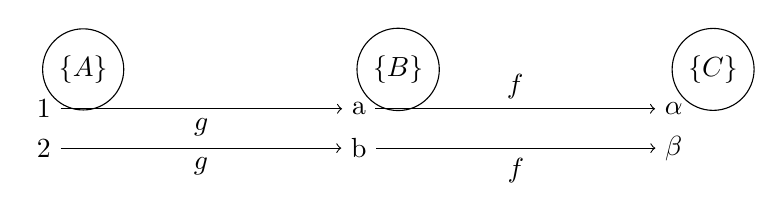
\begin{tikzpicture}[node distance=3cm, auto]
 % Nodes for the sets
  \node[circle, draw] (A) at (0,0) {$\{A\}$};
  \node[circle, draw] (B) at (4,0) {$\{B\}$};
  \node[circle, draw] (C) at (8,0) {$\{C\}$};

  
  % Elements in A
  \node (A1) at (-0.5,-0.5) {1};
  \node (A2) at (-0.5,-1) {2};

  % Elements in B
  \node (B1) at (3.5,-0.5) {a};
  \node (B2) at (3.5,-1) {b};

  % Elements in C
  \node (C1) at (7.5,-0.5) {$\alpha$};
  \node (C2) at (7.5,-1) {$\beta$};

  % Arrows for g
  \draw[->] (A1) to node [swap] {$g$} (B1);
  \draw[->] (A2) to node [swap] {$g$} (B2);

    % Arrows for f
  \draw[->] (B1) to node {$f$} (C1);
  \draw[->] (B2) to node [swap] {$f$} (C2);
\end{tikzpicture}
\quad
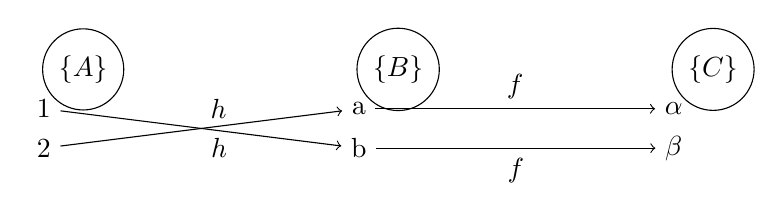
\begin{tikzpicture}[node distance=3cm, auto]
 % Nodes for the sets
  \node[circle, draw] (A) at (0,0) {$\{A\}$};
  \node[circle, draw] (B) at (4,0) {$\{B\}$};
  \node[circle, draw] (C) at (8,0) {$\{C\}$};

 

  % Elements in A
  \node (A1) at (-0.5,-0.5) {1};
  \node (A2) at (-0.5,-1) {2};

  % Elements in B
  \node (B1) at (3.5,-0.5) {a};
  \node (B2) at (3.5,-1) {b};

  % Elements in C
  \node (C1) at (7.5,-0.5) {$\alpha$};
  \node (C2) at (7.5,-1) {$\beta$};

  % Arrows for h
  \draw[->] (A1) to node {$h$} (B2);
  \draw[->] (A2) to node [swap] {$h$} (B1);

  % Arrows for f
  \draw[->] (B1) to node {$f$} (C1);
  \draw[->] (B2) to node [swap] {$f$} (C2);
\end{tikzpicture}
\end{center}

\begin{align*}
&\text{Given } f \text{ is a monomorphism, we have:} \\
&f \circ g(1) = f(a) = \alpha \\
&f \circ g(2) = f(b) = \beta \\
&f \circ h(1) = f(b) = \beta \\
&f \circ h(2) = f(a) = \alpha \\
&\text{If } f \circ g = f \circ h \text{, then } g = h \text{ as } f \text{ is left cancellative}.
\end{align*}




\section*{Epimorphisms in Category Theory}

\subsection*{Definition}
A morphism $f : A \rightarrow B$ in a category $\mathcal{C}$ is called an \textbf{epimorphism} (or \textbf{epi}) if for every pair of morphisms $g, h : B \rightarrow C$, the condition $g \circ f = h \circ f$ implies $g = h$.
\newline
In symbols:
\begin{equation*}
\forall g, h : B \rightarrow C, \quad (g \circ f = h \circ f) \implies (g = h)
\end{equation*}

\subsection*{Key Properties of Epimorphisms}
\begin{itemize}
    \item \textbf{Right Cancellative}: Epimorphisms are right cancellative. This means that if $g \circ f = h \circ f$ and $f$ is an epimorphism, then $g = h$.
    \item \textbf{Generalization of Surjective Functions}: In the category of sets, an epimorphism corresponds to a surjective (onto) function. However, in other categories, the notion of an epimorphism might not coincide with surjectivity in the usual sense.
    \item \textbf{Stability Under Composition}:
    \begin{itemize}
        \item If $f : A \rightarrow B$ and $g : B \rightarrow C$ are epimorphisms, then the composition $g \circ f : A \rightarrow C$ is also an epimorphism.
    \end{itemize}
\end{itemize}

\subsection*{Diagrams}
\subsubsection{External diagram}
Given that $f$ is an epimorphism,
\begin{equation*}
    g \circ f = h \circ f \implies g = h
\end{equation*}

\begin{center}
\begin{tikzpicture}[node distance=3cm, auto]
  % Nodes
  \node (A) at (0, 0) {$A$};
  \node (B) at (3, 2) {$B$};
  \node (C) at (6, 0) {$C$};

  % Arrows
  \draw[->] (A) to node [swap] {$f$} (B);
  \draw[->] (B) to node {$g$} (C);
  \draw[->] (B) to node [swap] {$h$} (C);

  % Arrow compositions
  \draw[->, dashed] (A) to node {$g \circ f$} (C);
  \draw[->, dashed] (A) to node [swap] {$h \circ f$} (C);
\end{tikzpicture}
\end{center}
\subsubsection{Internal Diagram}
Given that $f$ is a monomorphism,
\begin{equation*}
    f \circ g = f \circ h \implies g = h
\end{equation*}

\begin{center}
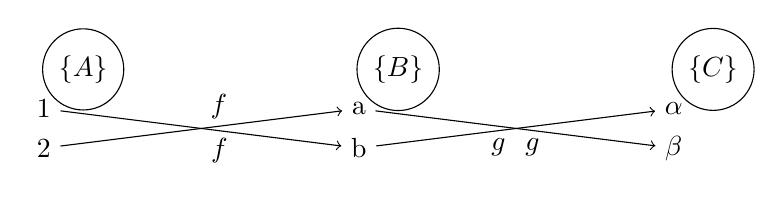
\begin{tikzpicture}[node distance=3cm, auto]
 % Nodes for the sets
  \node[circle, draw] (A) at (0,0) {$\{A\}$};
  \node[circle, draw] (B) at (4,0) {$\{B\}$};
  \node[circle, draw] (C) at (8,0) {$\{C\}$};

  
  % Elements in A
  \node (A1) at (-0.5,-0.5) {1};
  \node (A2) at (-0.5,-1) {2};

  % Elements in B
  \node (B1) at (3.5,-0.5) {a};
  \node (B2) at (3.5,-1) {b};

  % Elements in C
  \node (C1) at (7.5,-0.5) {$\alpha$};
  \node (C2) at (7.5,-1) {$\beta$};

  % Arrows for g
  \draw[->] (B1) to node [swap] {$g$} (C2);
  \draw[->] (B2) to node [swap] {$g$} (C1);

    % Arrows for f
  \draw[->] (A1) to node {$f$} (B2);
  \draw[->] (A2) to node [swap] {$f$} (B1);
\end{tikzpicture}
\quad
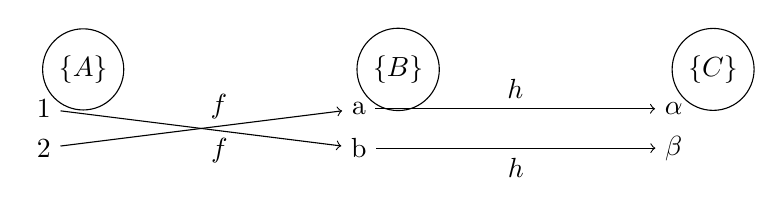
\begin{tikzpicture}[node distance=3cm, auto]
 % Nodes for the sets
  \node[circle, draw] (A) at (0,0) {$\{A\}$};
  \node[circle, draw] (B) at (4,0) {$\{B\}$};
  \node[circle, draw] (C) at (8,0) {$\{C\}$};

 

  % Elements in A
  \node (A1) at (-0.5,-0.5) {1};
  \node (A2) at (-0.5,-1) {2};

  % Elements in B
  \node (B1) at (3.5,-0.5) {a};
  \node (B2) at (3.5,-1) {b};

  % Elements in C
  \node (C1) at (7.5,-0.5) {$\alpha$};
  \node (C2) at (7.5,-1) {$\beta$};

  % Arrows for f
  \draw[->] (A1) to node {$f$} (B2);
  \draw[->] (A2) to node [swap] {$f$} (B1);

  % Arrows for h
  \draw[->] (B1) to node {$h$} (C1);
  \draw[->] (B2) to node [swap] {$h$} (C2);
\end{tikzpicture}
\end{center}

\begin{align*}
&\text{Given } f \text{ is a monomorphism, we have:} \\
&g \circ f(1) = g(b) = \alpha \\
&g \circ f(2) = g(a) = \beta \\
&h \circ f(1) = h(b) = \beta \\
&h \circ f(2) = h(a) = \alpha \\
&\text{If } g \circ f = h \circ f \text{, then } g = h \text{ as } f \text{ is right cancellative}.
\end{align*}







\end{document}
